\documentclass{standalone}
\usepackage{graphicx}	
\usepackage{amssymb, amsmath}
\usepackage{color}

\usepackage{tikz}
\usetikzlibrary{intersections, backgrounds, math}
\usepackage{pgfmath}

\definecolor{light}{RGB}{220, 188, 188}
\definecolor{mid}{RGB}{185, 124, 124}
\definecolor{dark}{RGB}{143, 39, 39}
\definecolor{highlight}{RGB}{180, 31, 180}
\definecolor{light_teal}{RGB}{107, 142, 142}
\definecolor{mid_teal}{RGB}{72, 117, 117}
\definecolor{dark_teal}{RGB}{29, 79, 79}
\definecolor{gray10}{gray}{0.1}
\definecolor{gray20}{gray}{0.2}
\definecolor{gray30}{gray}{0.3}
\definecolor{gray40}{gray}{0.4}
\definecolor{gray60}{gray}{0.6}
\definecolor{gray70}{gray}{0.7}
\definecolor{gray80}{gray}{0.8}
\definecolor{gray90}{gray}{0.9}
\definecolor{gray95}{gray}{0.95}

\begin{document}

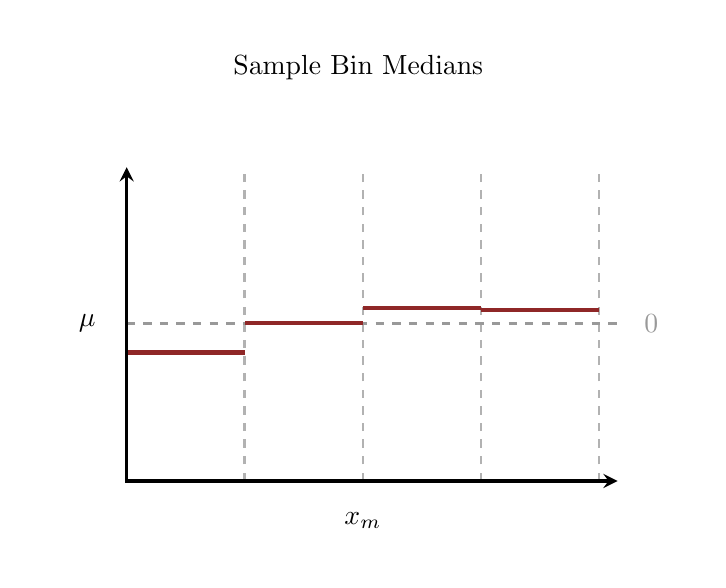
\begin{tikzpicture}[scale=1.0]

  \begin{scope}[shift={(17, 0)}]
    \draw[white] (-4.25, -3) rectangle (4.25, 3.75);
    
    \node[align=center] at (0, 3.25) { Sample Bin Medians };
    
    \foreach \b in {-3.0, -1.5,  0.0,  1.5,  3.0} {
      \draw[gray70, dashed, line width=1] (\b, -2) -- (\b, 2);
    }
    
    \draw[gray60, dashed, line width=1] (-3, 0) -- (3.25, 0);   
    \node[gray60, anchor=west] at (3.1, 0)  { $\quad 0$ };
    
    \foreach \l/\r/\m in {-3.000/-1.500/-0.368, -1.500/0.000/0.003, 
                          0.000/1.500/0.192, 1.500/3.000/0.170} {
       \draw[dark, line width=1.5] (\l, \m) -- (\r, \m);
    }
     
    \draw [->, >=stealth, line width=1.25] (-3.00, -2.015) -- +(0, 4);
    \draw [->, >=stealth, line width=1.25] (-3.015, -2.00) -- +(6.25, 0);
    
    \node at (-3.5, 0) { $\mu$ };
    \node at (0, -2.5) { $x_{m}$ };
  \end{scope}
    
\end{tikzpicture}

\end{document}  